\chapter{Searching for Long Lived Particles}

This chapter presents some context about searches for \acp{LLP}, including basic concepts of particle decay, as well as advantages and challenges of unconventional searches.

In the context of \ac{ATLAS}, a particle is \emph{long lived} if information about its lifetime can be inferred using the detector. A \ac{LLP} can decay somewhere inside of the detector and a signature of this decay observed, or it can be stable with repsect to the detector and never decay inside of it. This is contrasted with \emph{promptly decaying} particles, which decay into \emph{detector stable} particles before reaching the detector. An overview of various \ac{LLP} signatures used in \ac{BSM} searches is also presented.

\section{Lifetime}
%USED theory-llp-whitepaper.pdf
Any particle's lifetime is given as the inverse of its \emph{width}:

\begin{equation}
\tau = \frac{1}{\Gamma}
\end{equation}

Where its width can be defined as:

\begin{equation}
\Gamma = \frac{1}{2m_{X}} \int d\Pi_f \big| \mathcal{M}(m_X \rightarrow \{p_f\})\big|^2
\end{equation}

where $m_X$ is the mass of the particle, $\mathcal{M}$ is the matrix element for the particle's decay into its decay products $\{p_f\}$ and $d\Pi_f$ is the Lorentz-invariant phase space of the decay. 

A particle can decay in several different ways, in which case width for various process is summed to calculated the particle's \emph{total width}. It is the inverse of the total width that governs the particle's lifetime.

In order for the lifetime of a particle to be long, the width must be small, meaning that the matrix element or allowed phase space must be small. A small matrix element can be caused by a small coupling, and a small phase space can be caused by almost-degenerate mass spectra (like a muon) or very offshell intermediate states (like a neutron). All of which are common in both the \ac{SM} and many \ac{BSM} theories. The range of liftimes of \ac{SM} particles can be seen in \autoref{fig:llp-mass-lifetime}


\begin{figure}[htbp]
\centering
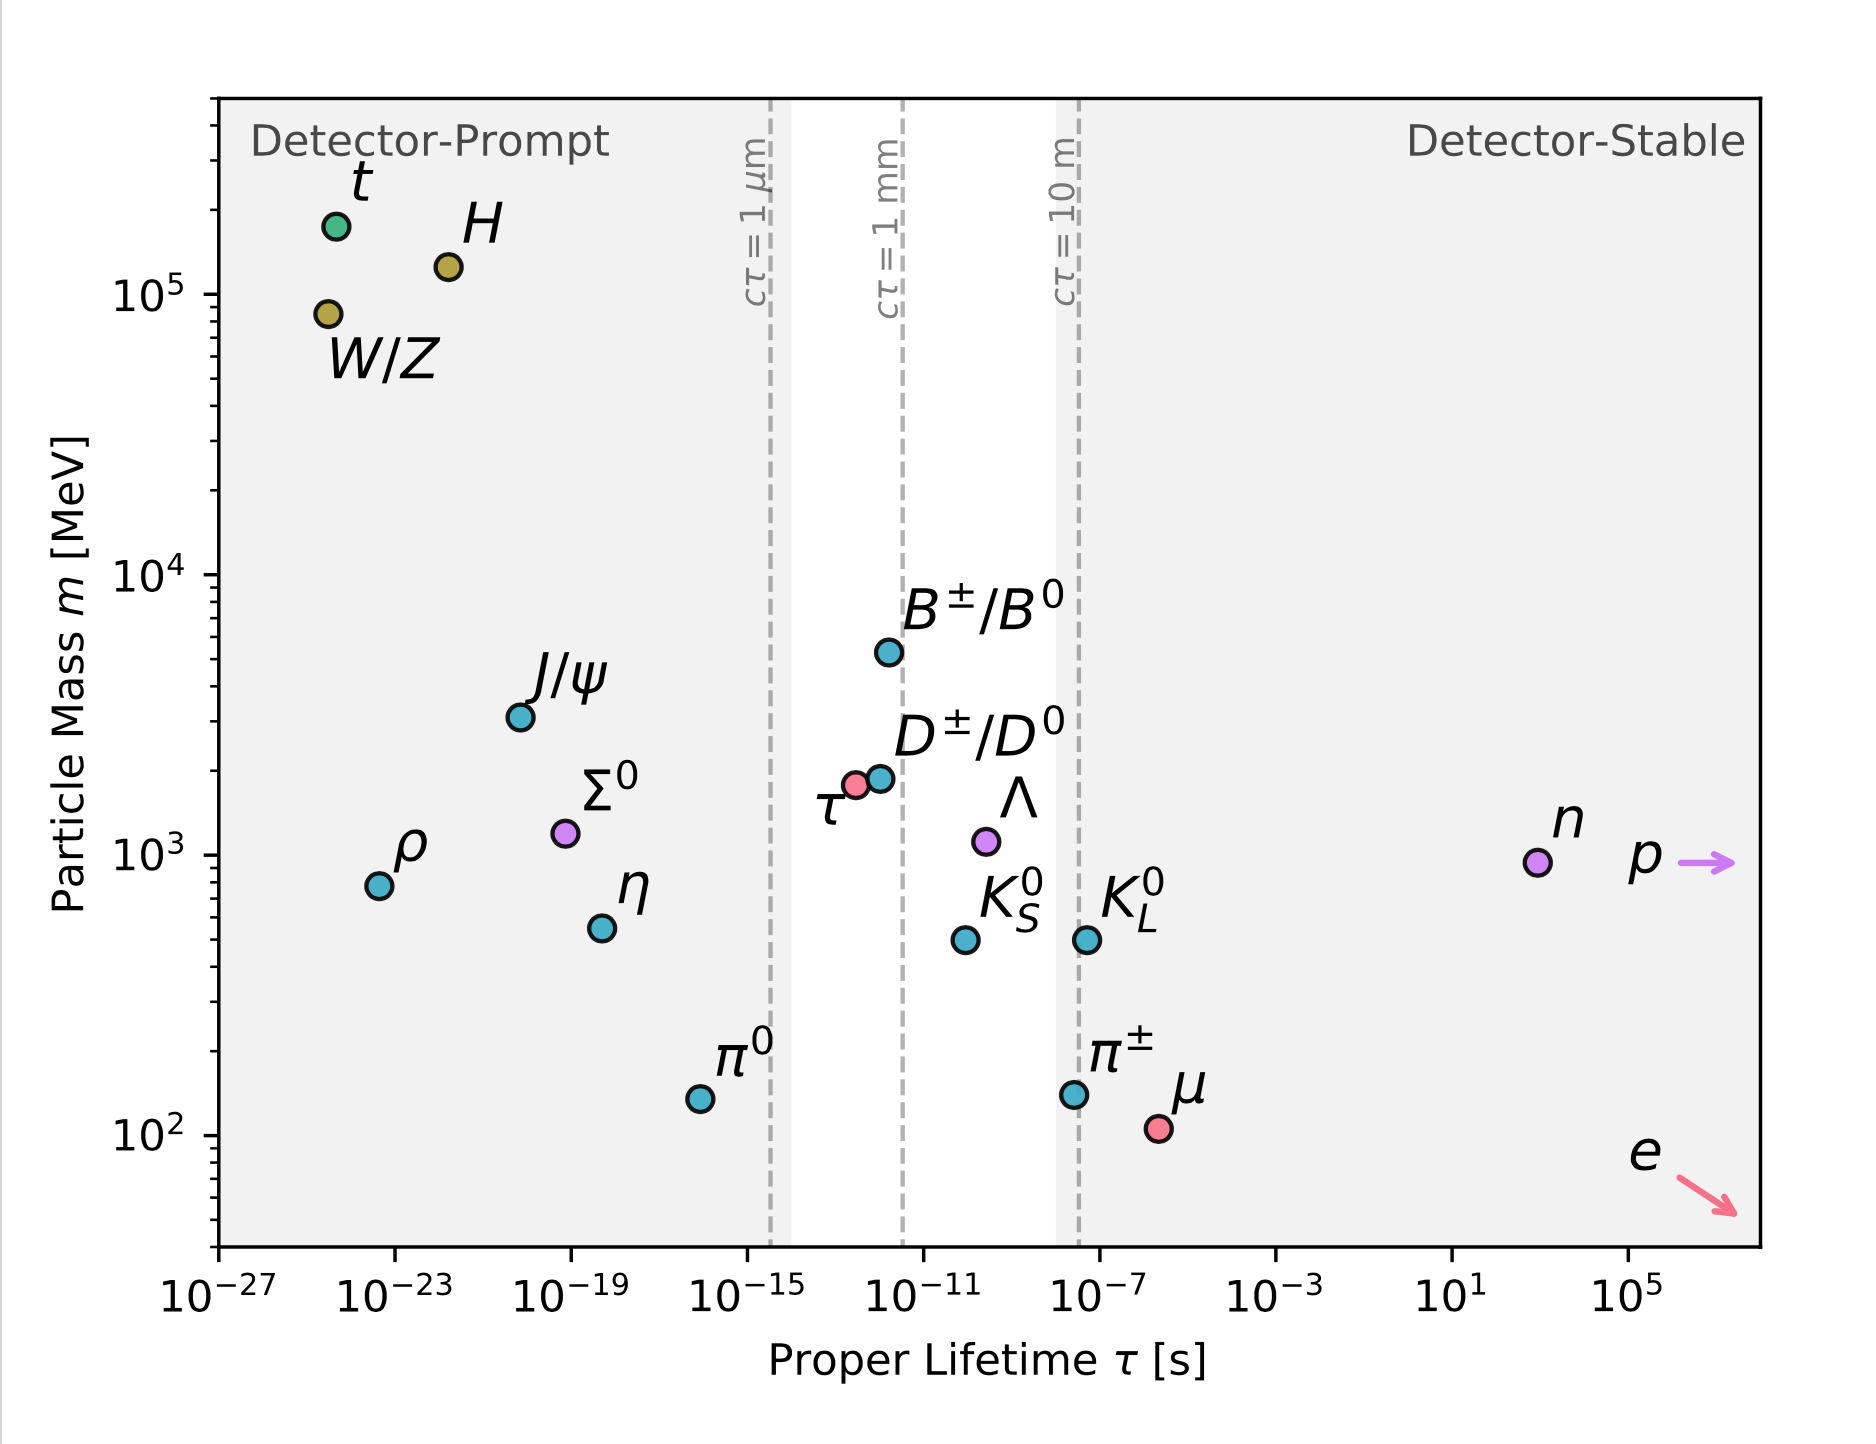
\includegraphics[width=.8\textwidth]{figures/theory/LLP-mass-lifetime.png}
\caption{A mass and proper lifetime distribution of particles in the \ac{SM}. There is a wide range of both masses and lifetimes. Shaded regions indicate detector-prompt or detector-stable particles. This assumes that particles traveling at the speed of light $\beta = 1$.}
\label{fig:llp-mass-lifetime}
\end{figure}

\section{Particle Decays}
%USED theory-LLP-Banerjee.pdf

The distance traveled by any relativistic particle can be described by

\begin{equation}
d = vt = \beta \gamma c t
\label{eq:sr_d}
\end{equation}

where $\gamma$ and $\beta$ have the usual special relativistic definitions: $\gamma = E/m = (1-\beta^2)^(-1/2)$, $\beta = v/c = |\vec{p}|/E$, $v$ is the particle's velocity, $t$ is the time the particle moves, and $c$ is the speed of light 

In the laboratory frame, the distance the particle travels before decaying is given by sending $t \rightarrow \tau$ in \autoref{eq:sr_d}, where $\tau$ denotes the proper lifetime of the particle measured in its own rest frame.

There is an exponential probability that the particle will decay at a given time ($t$) and location ($x$), given by 

\begin{equation}
P(x) = e ^{-x/(\beta \gamma \tau)}
\end{equation}

This means that even particles with large $\tau$ have a large probability at traveling very small distances before they decay, but particles with small $\tau$ cannot travel large distances before decaying. This fact is exploited to search for particles with large $\tau$, though the signature of the particle's decay in the detector varies greatly with the size of $\tau$. The relationship between decay radius and lifetime can be seen in \autoref{fig:d0-rltns}.


\section{\label{sec:llp-searches}Searches for Long Lived Particles}

\todo{need to hunt down papers and add references in the below}

\todo{Maybe add a doodle? Seperate doodles for each signature to just just copy heather's diagram?}

If more than one of the products of the \ac{LLP} decay are visible to the detector, one can look for its decay vertex. The \ac{LLP} will travel some distance from the \ac{PV}, where the particle is produced, and its decay vertex will be displaced, called a \ac{DV}. In this case, direct information about the lifetime of the particle can be deduced from the difference in distance between the \ac{LLP}'s prodcution and decay vertices (given by \autoref{eq:sr_d}). This vertices can appear in either tracking volume of the detector (\ac{ID} or \ac{MS}). There are many searches for \ac{DV}s in \ac{ATLAS}, many in conjunction with other physics objects related to the particlar theory model being probed. 

One can also directly search for the \ac{LLP}. In these cases, the \ac{LLP} is charged and leaves a peculiar track in the \ac{ID}. For example, one can look for highly ionizing tracks, indicating the presence of a massive particle that does not decay inside the \ac{ID} or for short tracks, where the decay products of the \ac{LLP} are not detected.

Finally, as in the case of this analysis, one can look for only the decay products of the \ac{LLP} by targetting  unconventionally presenting physics objects. For example, look for non-pointing photons in the \ac{LAr}, or emerging jets, which become visible midway through their hadronization. One can also look for displaced leptons, somewhat conventional lepton signtures that do not point back to the \ac{PV}. 

In these cases, it is often convenient to use \dzero, the transverse impact parameter, as a way to infer the lifetime of a particle. It does not give direct information about $\tau$, but decay products of particles with longer lifetimes have wider \dzero distributions as seen in \autoref{fig:d0-rltns}. In cases without a \ac{DV}, \dzero gives more precise information than any $R$ information realted to the track of the decay product. \dzero is calculated based on the shape of the track and has $\mathcal{0}(10)\mu \textrm{m}$ resolution (see \autoref{fig:trking_d0_res}). In $R$, we can only know the location of the first \ac{ID} layer associated to the track, with an $\mathcal{0}(10)\textrm{mm}$ resolution very sensitive to detector effects.

\todo{make a LLP decay diagram, also with different \pt}

\begin{figure}[htbp]
\centering
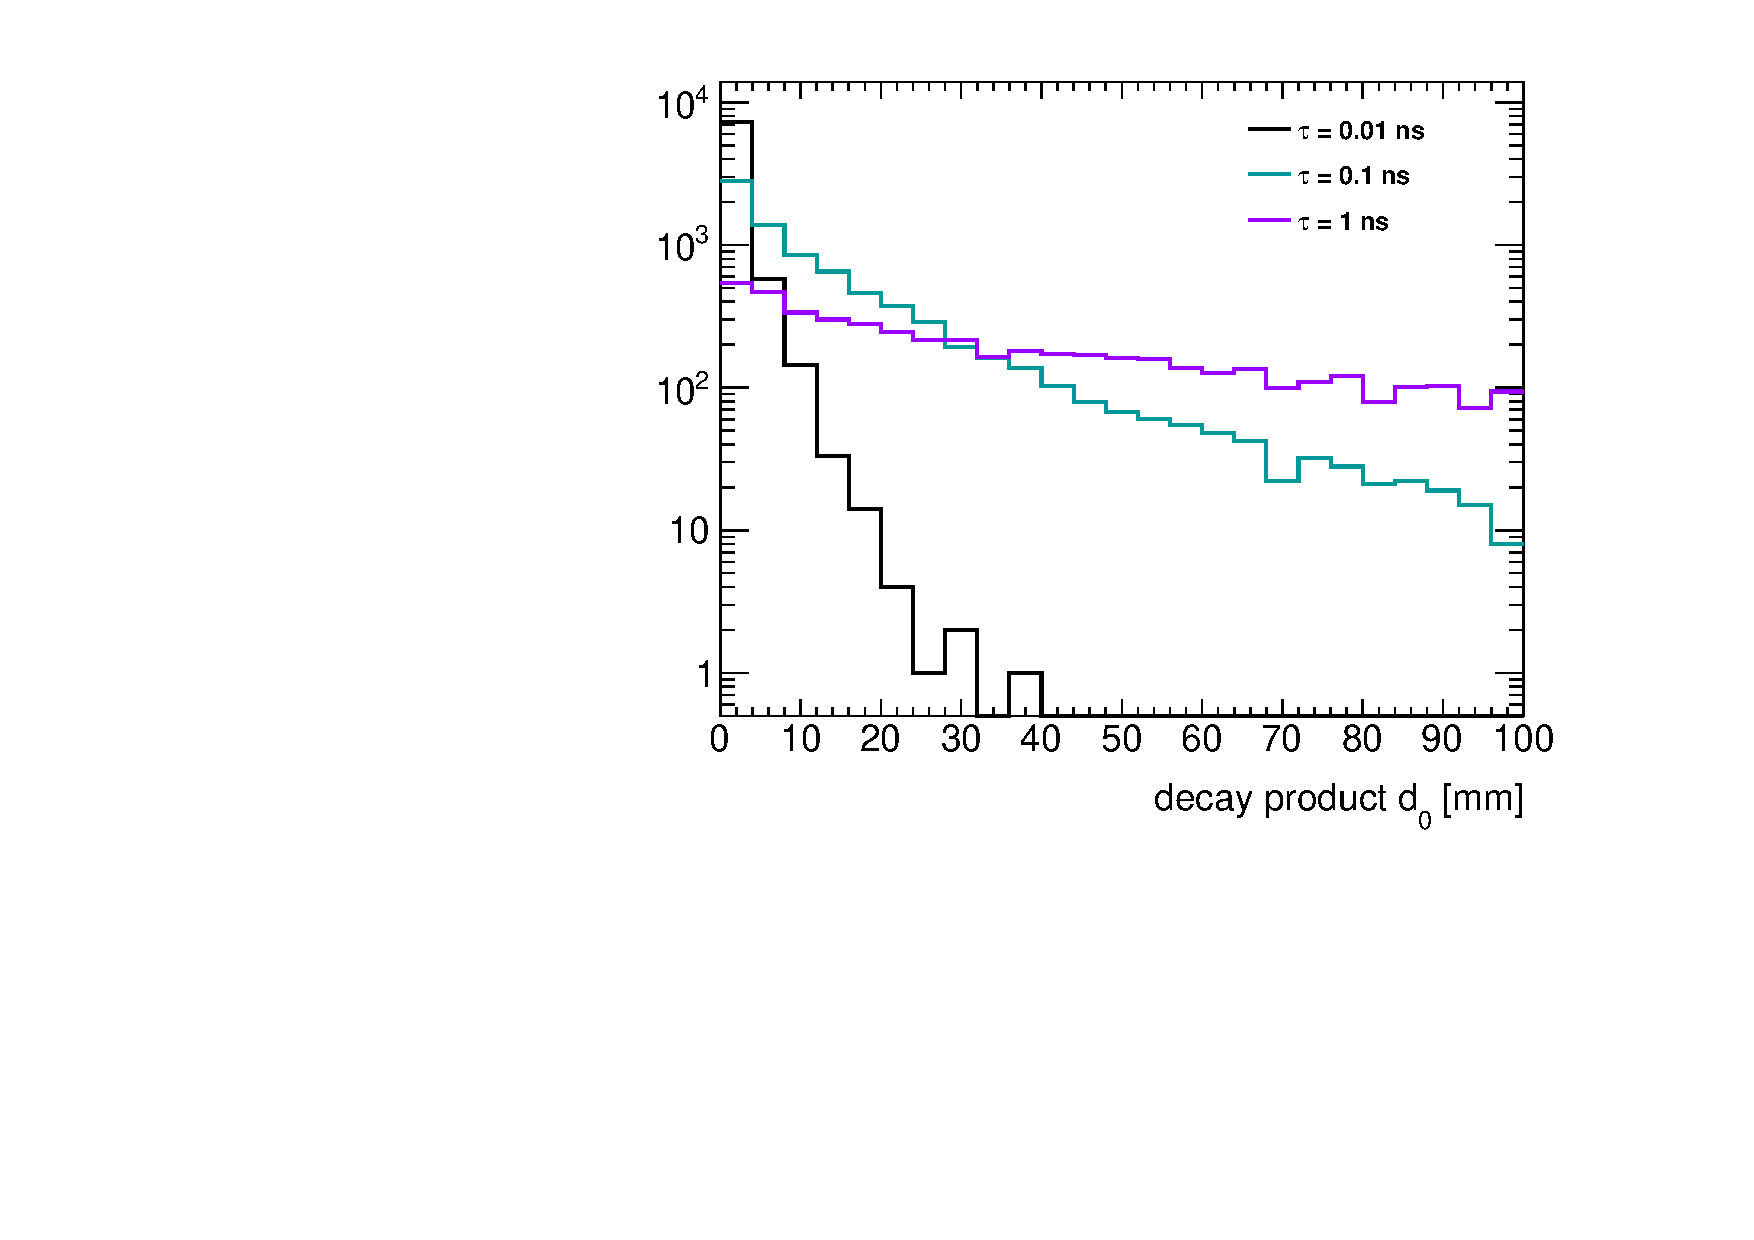
\includegraphics[width=.48\textwidth]{figures/theory/signal_d0.pdf}
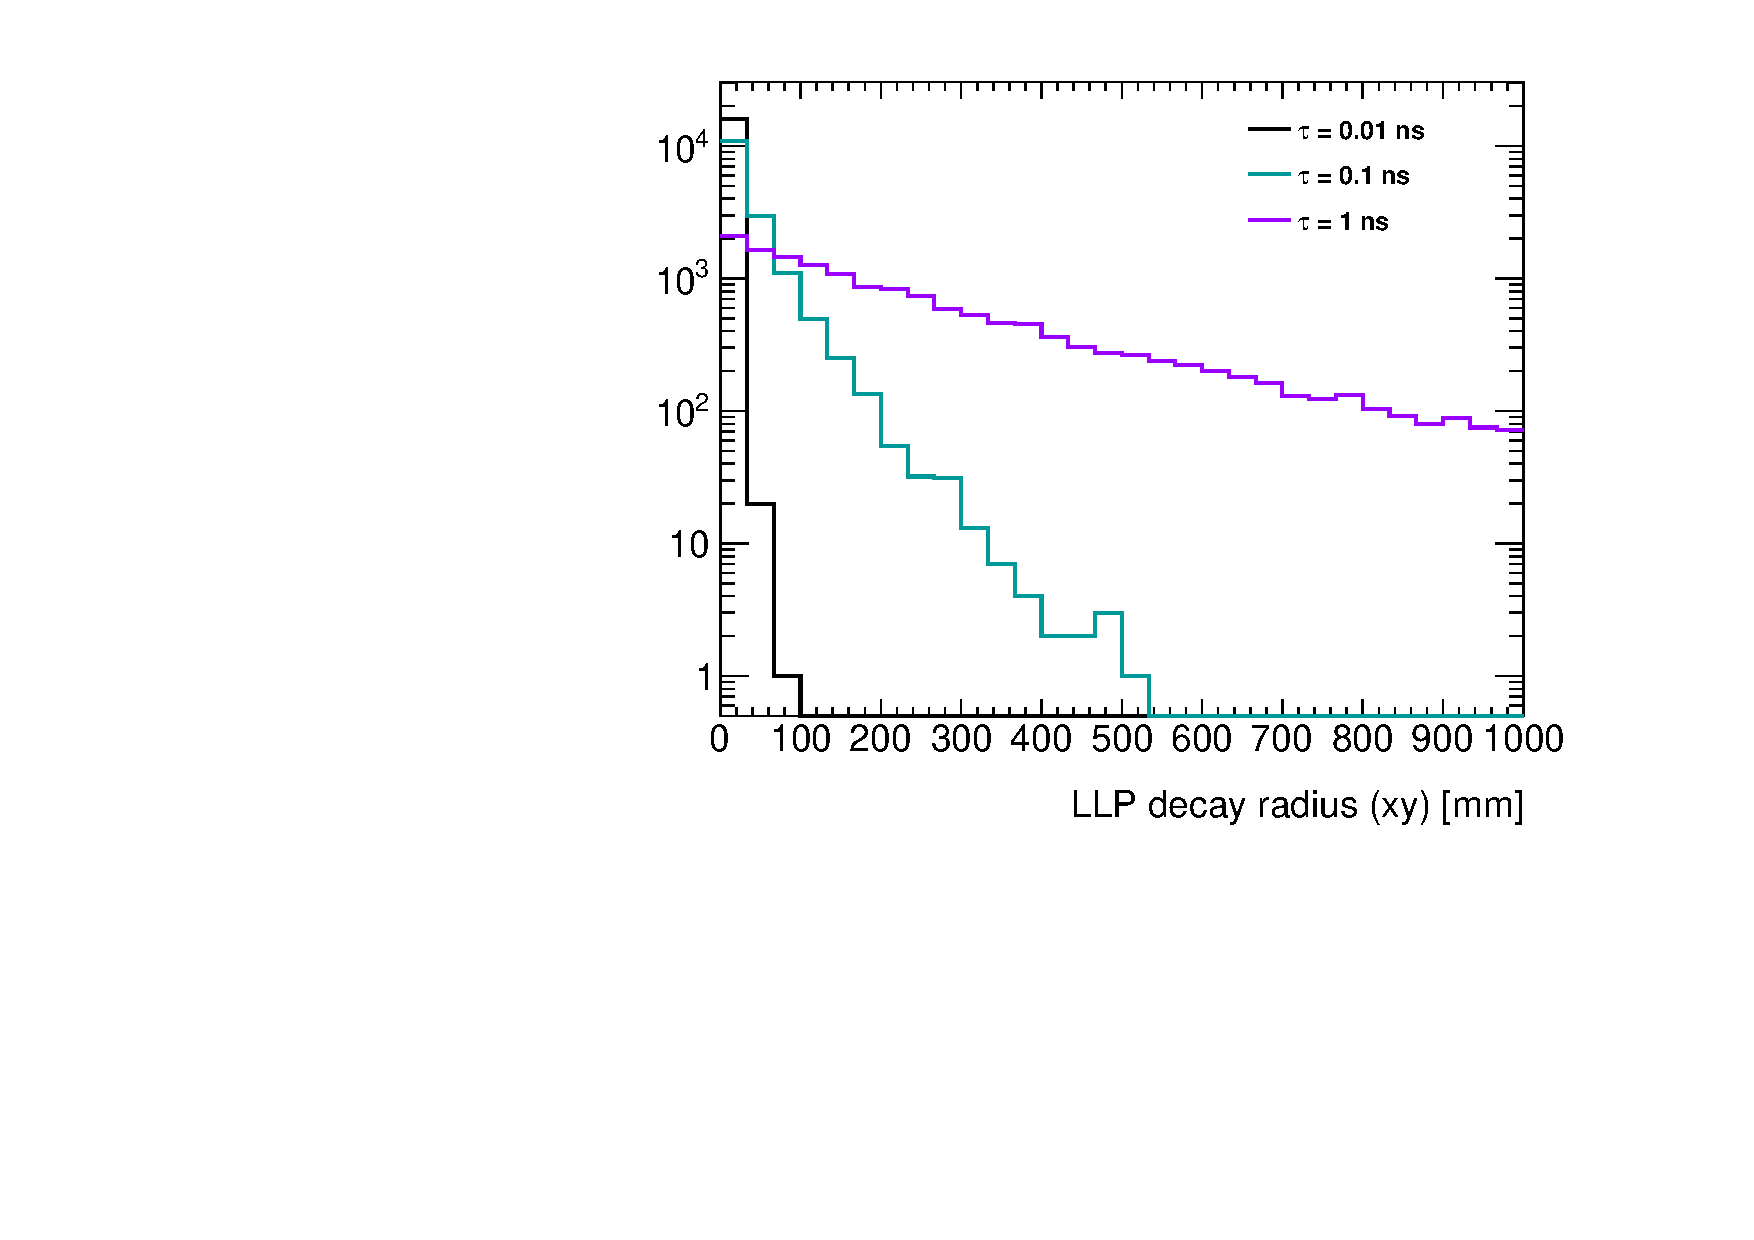
\includegraphics[width=.48\textwidth]{figures/theory/signal_rxy.pdf}
\caption{\dzero (left) and transverse decay radius ($x-y$) of \ac{LLP}s with different $\tau$. The left plot demonstrates that while \dzero does not directly give information about $\tau$, decay products of particles with longer lifetimes have wider \dzero distributions. These plots demonstrate only effects of the physical processes, not convolved with reconstrution effects.}
\label{fig:d0-rltns}
\end{figure}


These signatures are very unique with respect to other signatures searched for in \ac{ATLAS} which generally assume decay products originate at the \ac{PV}. These searches are dominated by \ac{SM} \emph{backgrounds}, physical phenomena that are not the target for measurement but have very similar signatures. \ac{LLP} searches generally have very little \ac{SM} background, but suffer from reconstruction challenges.A great deal of work is put into efficient and pure reconstruction and identification of unconventional physics objects.

Due to the technical challenges associated with \ac{LLP} searches, they are often done to be as \emph{model-independent} as possible. This means that, while there is usually a model to which a search brings unique sensitivity, the search not overoptimized for this model. For example, in this analysis, we target the displaced leptons; there are other objects in the targetting physical process, but we remain agnostic to them. Furthermore, the exponetial nature of the \ac{LLP} decay means that several searches, each targetting different signatures in different parts of the detector, are used in combination to explore the full lifetime phase space of a given model.


\todo{implications of 0 background search, why are 3 events required for discovery?}


